\documentclass{standalone}
\usepackage{pgfplots}
\pgfplotsset{compat=newest}

\begin{document}
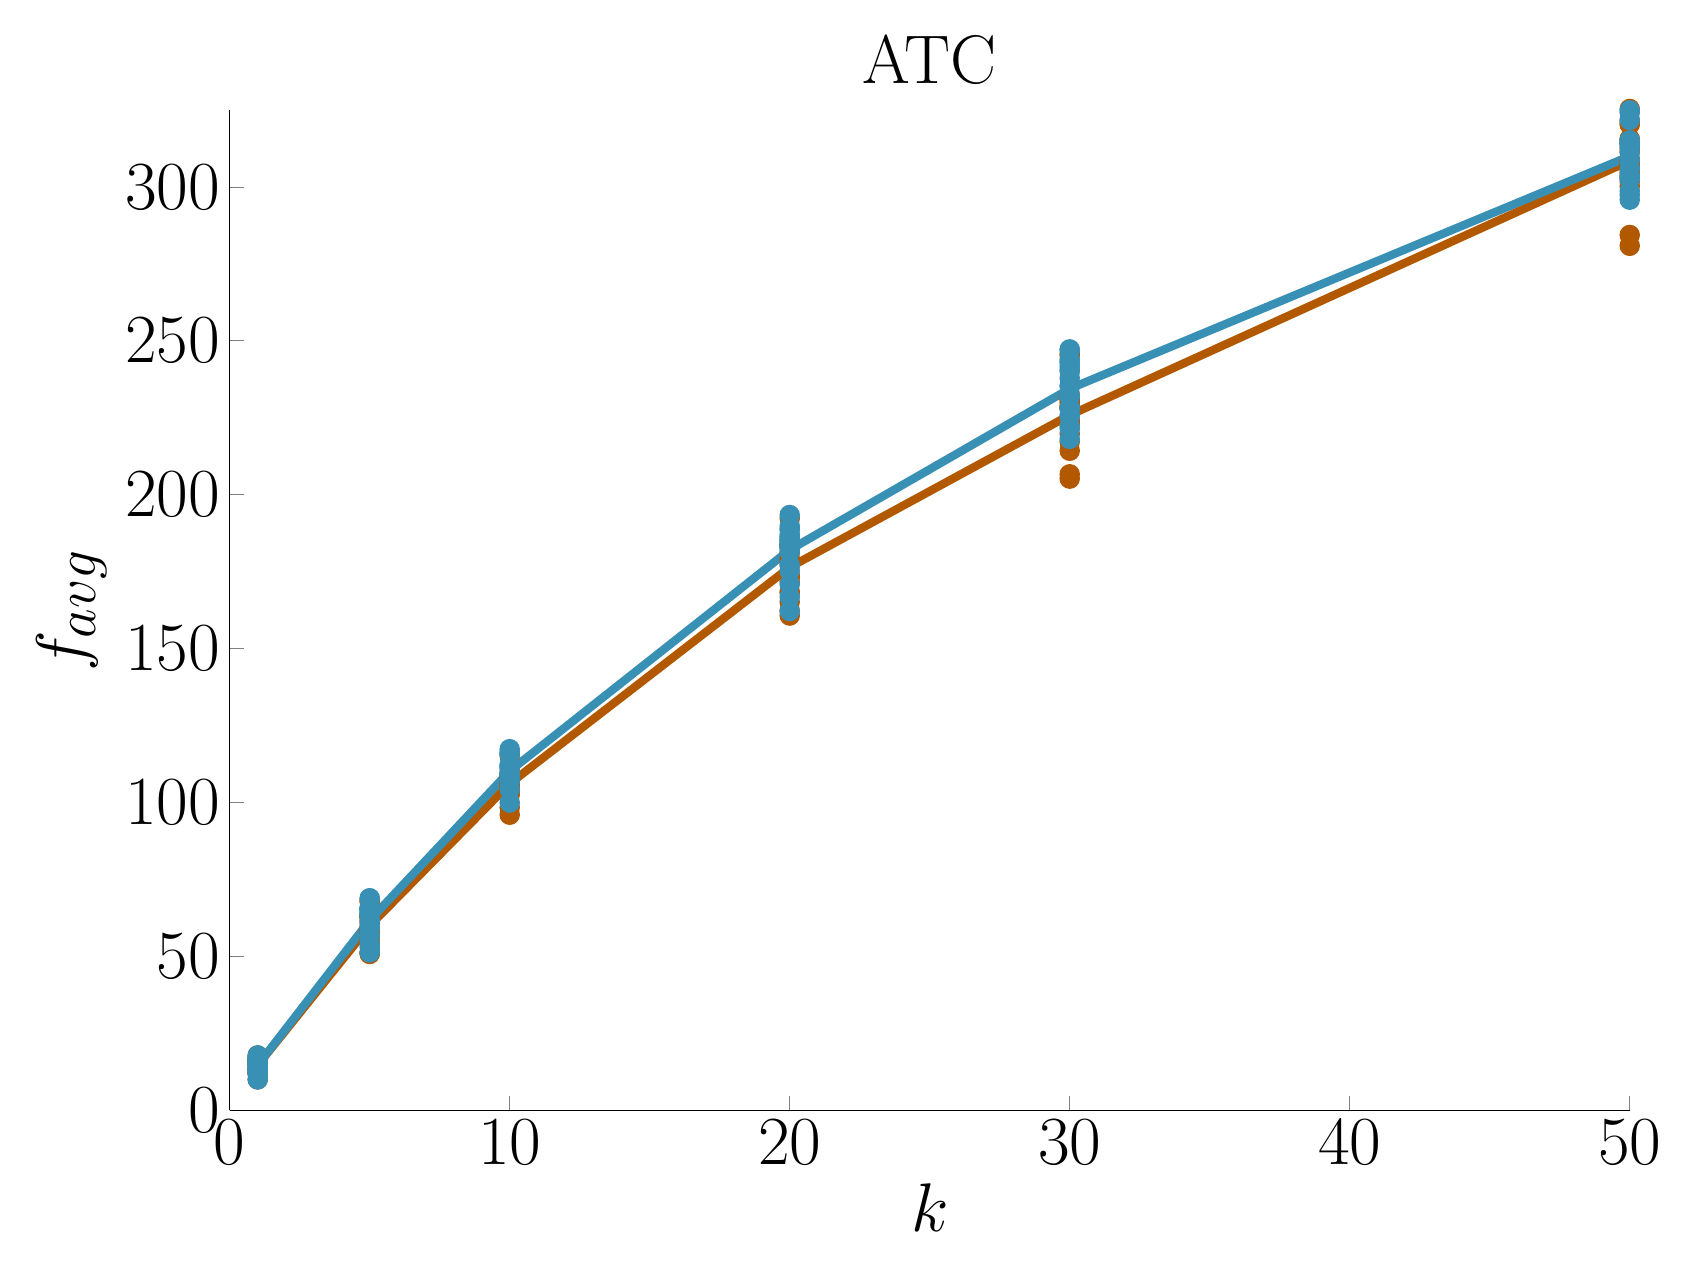
\begin{tikzpicture}

\begin{axis}[%
title style={font=\Huge},
title=ATC,
tick label style={font=\Huge},
label style={font=\Huge},
legend style={font=\Huge},
view={0}{90},
max space between ticks=50pt,
width=7in,
height=5in,
scale only axis,
xmin=0, xmax=50,
xtick={0, 10, 20, 30, 40, 50},
xlabel={$k$},
ymin=0, ymax=324.87,
%ytick={0, 200, 400, 600, 800, 1000},
ylabel={$f_{avg}$},
major tick length=5pt,
axis lines*=left,
legend cell align=left,
clip=false]

\addplot [
only marks,
mark=*,
mark size=3.5pt,
color=orange!70!black,
%solid,
%line width=2pt,
]
coordinates{
(1,10.04)(1,11.86)(1,12.14)(1,12.87)(1,13.1)(1,13.38)(1,13.7)(1,13.72)(1,14.82)(1,15.1)(1,15.11)(1,15.2)(1,15.42)(1,15.66)(1,16.22)(1,16.42)(1,16.44)(1,16.81)(1,17.09)(1,17.83)(5,50.79)(5,51.11)(5,51.21)(5,54.56)(5,55.83)(5,57.43)(5,58.36)(5,59.17)(5,59.49)(5,60.71)(5,61.55)(5,62.48)(5,62.57)(5,62.93)(5,63.11)(5,63.27)(5,63.41)(5,65.28)(5,67.82)(5,68.01)(10,96.03)(10,98.43)(10,102.56)(10,103.29)(10,104.34)(10,104.56)(10,105.04)(10,105.33)(10,106.08)(10,106.47)(10,107.17)(10,107.56)(10,107.81)(10,107.96)(10,108.3)(10,108.37)(10,108.81)(10,109.05)(10,110.15)(10,115.16)(20,160.73)(20,162.32)(20,165.18)(20,168.12)(20,168.4)(20,171.75)(20,173.3)(20,173.51)(20,173.87)(20,177.06)(20,178.3)(20,179.38)(20,181.18)(20,182.97)(20,183.39)(20,183.45)(20,183.71)(20,183.96)(20,185.36)(20,192.36)(30,205.21)(30,206.62)(30,214.26)(30,217.15)(30,219.77)(30,223.15)(30,223.43)(30,223.99)(30,224.08)(30,227.96)(30,228.15)(30,228.43)(30,228.56)(30,229.68)(30,230.46)(30,231.04)(30,231.37)(30,232.49)(30,245.3)(30,245.79)(50,280.85)(50,284.37)(50,300.19)(50,301.63)(50,303.46)(50,304.49)(50,305.21)(50,306.89)(50,307.5)(50,308.44)(50,309.09)(50,311.57)(50,312.36)(50,314.75)(50,315.42)(50,315.58)(50,320.27)(50,320.56)(50,321.58)(50,325.3)
};

\addplot [
only marks,
mark=*,
mark size=3.5pt,
color=cyan!70!black,
%solid,
%line width=2pt,
]
coordinates{
(1,10.04)(1,11.86)(1,12.14)(1,12.87)(1,13.1)(1,13.38)(1,13.7)(1,13.72)(1,14.82)(1,15.1)(1,15.11)(1,15.2)(1,15.42)(1,15.66)(1,16.22)(1,16.42)(1,16.44)(1,16.81)(1,17.09)(1,17.83)(5,51.29)(5,52.9)(5,53.89)(5,56.67)(5,56.78)(5,59.42)(5,59.78)(5,61.34)(5,63.14)(5,63.16)(5,63.44)(5,63.88)(5,64.31)(5,64.67)(5,65.23)(5,65.52)(5,65.56)(5,65.85)(5,68.86)(5,68.87)(10,99.98)(10,104.25)(10,107.01)(10,107.44)(10,107.49)(10,108.62)(10,108.8)(10,109.06)(10,109.18)(10,109.24)(10,109.44)(10,111.05)(10,111.45)(10,111.67)(10,111.93)(10,112.36)(10,115.63)(10,116.13)(10,116.33)(10,117.32)(20,162.18)(20,166.78)(20,170.89)(20,175.33)(20,177.19)(20,181.45)(20,182.43)(20,182.89)(20,183.48)(20,183.81)(20,184.26)(20,185.12)(20,185.16)(20,186.2)(20,186.29)(20,187.06)(20,188.76)(20,188.78)(20,189.83)(20,193.4)(30,218.12)(30,221.39)(30,222.09)(30,225.46)(30,225.91)(30,227.94)(30,228.25)(30,231.86)(30,232.41)(30,235.1)(30,235.39)(30,237.9)(30,240.09)(30,240.56)(30,241.62)(30,242.86)(30,243.22)(30,243.96)(30,247.03)(30,247.21)(50,295.83)(50,297.37)(50,298.65)(50,302.51)(50,302.83)(50,303.14)(50,303.76)(50,306.0)(50,308.8)(50,311.11)(50,312.97)(50,313.87)(50,313.89)(50,314.04)(50,314.04)(50,314.89)(50,315.1)(50,321.73)(50,324.12)(50,324.87)
};

\addplot [
color=orange!70!black,
solid,
line width=3pt
]
coordinates{
(1,14.6465)(5,59.9545)(10,106.1235)(20,176.415)(30,225.8445)(50,308.4755)
};

\addplot [
color=cyan!70!black,
solid,
line width=3pt
]
coordinates{
(1,14.6465)(5,61.728)(10,110.219)(20,182.0645)(30,234.4185)(50,309.976)
};


\end{axis}
\end{tikzpicture}
\end{document}
